\FloatBarrier

\begin{figure}[h!]
\centering
\caption{Full-Wave Bridge Rectifier Circuit}
\label{fig:fwr}
\begin{circuitikz}
	\draw
	( 0 , 4 ) to [ sV , v<=$20Vpp$ ] ( 0 , 0 )
	( 0 , 4 ) -- ( 4 , 4 ) to [ empty diode ] ( 6 , 2 )
	( 2 , 2 ) to [ empty diode ] ( 4 , 4 )
	( 2 , 2 ) to [ empty diode ] ( 4 , 0 )
	( 4 , 0 ) to [ empty diode ] ( 6 , 2 )
	( 4 , 0 ) -- ( 0 , 0 )
	( 2 , 2 ) to [ R = 300 <\ohm> ] ( 6 , 2 )
	( 2 , 2 ) node[label={ [font=\normalsize] above : $-$ } ] { }
	( 6 , 2 ) node[label={ [font=\normalsize] above : $+$ } ] { }
	;
\end{circuitikz}
\end{figure}

\FloatBarrier

Figure (\ref{fig:fwr}) displays a full-wave bridge rectifier circuit. The circuit's specification requires that it take an input sinusoidal signal and produce an output voltage that is the absolute value of that signal with the least amount of error possible. The output voltage is measured over the resistor, which shall be referred to as $R$. In reality, this ideal is not reached. The experiment demonstrates the degree to which the specification is satisfied.
The full-wave bridge rectifier circuit takes advantage of the fact that diodes essentially act as broken circuits when the applied voltage is less than its threshold voltage and act as short circuits when the applied voltage exceeds its threshold voltage. This is a simplification of the Shockley diode model:

\begin{equation}
	\label{eq:shockley_diode}
	I_{diode}( V_{applied} ) = I_0 ( e^{ \frac{qV_{applied}}{k_B T} } - 1 )
\end{equation}

In equation (\ref{eq:shockley_diode}), $I_0$ is the reverse saturation current, $q$ is the elementary charge, $k_B$ is Boltzmann's constant, and $T$ is temperature. A more ideal model treats the diode as the perfect switch described above, namely that the diode acts as a broken circuit unless $V_{applied}$ exceeds its threshold voltage, assumed to be about 0.7\si{\volt} and referred to as $V_{Th}$. Figure (\ref{fig:ideal_vs_shock}) below compares these two models in a graph. The graph demonstrates that this more idealized model accurately characterizes the behavior of the diode. It shall be used instead to describe the diode's characteristics.

\FloatBarrier

\begin{figure}[h!]
	\centering
	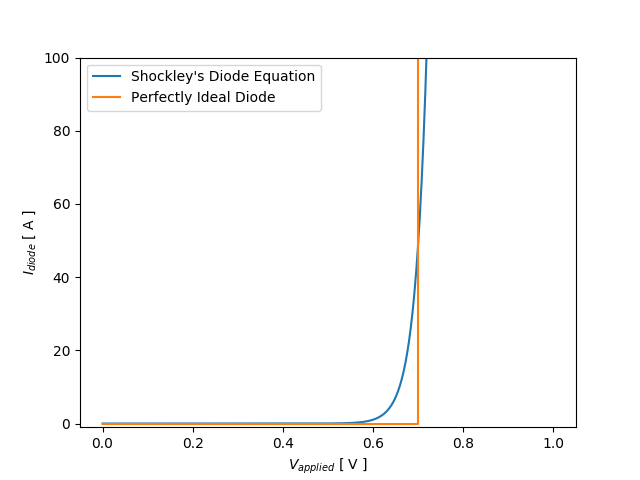
\includegraphics[scale=0.75]{../images/ideal_diode.PNG}
	\caption{Shockley Diode Model vs. Perfectly Ideal Diode}
	\label{fig:ideal_vs_shock}
\end{figure}

\FloatBarrier

{\footnotesize $I_0$ is set to 0.1\si{\nano\ampere}. Temperature is assumed to be 300\si{\kelvin}. Threshold voltage of perfectly ideal model is assumed to be 0.7\si{\volt}. }

\FloatBarrier

A diode is said to be enabled when the applied source voltage, which shall be called $V_{A}$, meets or exceeds its threshold voltage. Enabled diodes are drawn in green. Two cases are to be considered: when $V_{A} > 2V_{Th}$ and when $V_{A} < 2V_{Th}$. $2V_{Th}$ must be used since the voltage must enabled two diodes in series as seen in the figures below. Note that $|V_{A}| < 2V_{Th}$ is trivial since no voltage drops over the load resistor $R$.

When $V_{A} > 2V_{Th}$, the diodes in figure (\ref{fig:v_app_high}) are enabled. The voltage measured over the resistor is clearly positive due to the direction of positive current flow. The positive current flow direction is indicated by an arrow.

\FloatBarrier

\begin{figure}[h!]
\centering
\caption{Full-Wave Rectifier when $V_{applied} > 0$}
\label{fig:v_app_high}
\begin{circuitikz}
	\draw
	( 0 , 4 ) to [ sV , v<=$20Vpp$ ] ( 0 , 0 )
	( 0 , 4 ) -- ( 4 , 4 ) to [ empty diode , color = green ] ( 6 , 2 )
	( 2 , 2 ) to [ empty diode ] ( 4 , 4 )
	( 2 , 2 ) to [ empty diode , color = green ] ( 4 , 0 )
	( 4 , 0 ) to [ empty diode ] ( 6 , 2 )
	( 4 , 0 ) -- ( 0 , 0 )
	( 2 , 2 ) to [ R = 300 <\ohm> , i<_=$I$ ] ( 6 , 2 )
	( 2 , 2 ) node[label={ [font=\normalsize] above : $-$ } ] { }
	( 6 , 2 ) node[label={ [font=\normalsize] above : $+$ } ] { }
	;
\end{circuitikz}
\end{figure}

\FloatBarrier

Figure (\ref{fig:v_app_low}) demonstrates the case when $V_{A} < 2V_{Th}$. Again, the output voltage taken over the resistor is positive due to the direction of positive current flow.

\FloatBarrier

\begin{figure}[h!]
\centering
\caption{Full-Wave Rectifier when $V_{applied} > 0$}
\label{fig:v_app_low}
\begin{circuitikz}
	\draw
	( 0 , 4 ) to [ sV , v<=$20Vpp$ ] ( 0 , 0 )
	( 0 , 4 ) -- ( 4 , 4 ) to [ empty diode ] ( 6 , 2 )
	( 2 , 2 ) to [ empty diode , color = green ] ( 4 , 4 )
	( 2 , 2 ) to [ empty diode ] ( 4 , 0 )
	( 4 , 0 ) to [ empty diode , color = green ] ( 6 , 2 )
	( 4 , 0 ) -- ( 0 , 0 )
	( 2 , 2 ) to [ R = 300 <\ohm> , i<_=$I$ ] ( 6 , 2 )
	( 2 , 2 ) node[label={ [font=\normalsize] above : $-$ } ] { }
	( 6 , 2 ) node[label={ [font=\normalsize] above : $+$ } ] { }
	;
\end{circuitikz}
\end{figure}

\FloatBarrier

In the
